\cotefile{10}
\scanpage{102}
\mspage{101}

Quelques exemples de catégories tensorielles.

1) Soit $M$ un groupe. Soit $\underline{C}_M$\rlap{\handwritten{\tikz[baseline=0pt,x=1em,y=1em]{\draw (0,1.25)--(.4,-.65);}}} la catégorie des vectoriels de dimension finie sur le corps $k$, munis d'une graduation de type $M$. C'est une catégorie tensorielle sur $k$, munie d'un foncteur fibre sur $k$, le foncteur ``\unsure{oublif|oublie|oubli} de la graduation''. Le groupe algébrique associé est le groupe de type multiplicatif $D_k(M)$ (SGA 3 I 4.7.3). Par exemple si $M=\underline{Z}^r$, on trouve $G=\underline{G}_m^r$.

Application: soit $\underline{C}$ une catégorie tensorielle sur $k$ munie d'un foncteur fibre \inserted{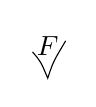
\begin{tikzpicture}[baseline=-.1ex,x=1em,y=1em]\node at (0,.9) {$F$};\draw (-.55,.7) .. controls (-.25,.35) .. (0,-.25) .. controls (.2,.35) .. (.65,1.1);\end{tikzpicture}} sur $k$, donc associée à un schéma en groupes affine $G$ sur $k$\unsure{.|,} On cherche toutes les façons de mettre, pour chaque $M\handwritten{\in}\operatorname{Ob}\underline{C}$, une graduation de type $M$ sur $F(V)$, de façon fonctorielle en $M$, et compatible (dans un sens évident) avec les produits tensoriels.Ell\unsure{\rlap{l}e|e}s correspondent aux $\otimes$-foncteurs de $\underline{C}$ dans $\underline{C}_M$ compatibles avec les foncteurs fibres, donc aux homomorphismes de $D_k(M)$ dans $G$. Par exemple, si $M=\underline{Z}^r$, il faut prendre les homomorphismes de $\underline{\unsure{G|E|\mathbb{G}}}_m^r$ dans $G$.

Dans la situation précédente, on peut se demander quand une $\otimes$-graduation de type $M$ du foncteur $F$ correspond à une graduation de type $M$ du foncteur identique de $\underline{C}$, i.e. pour tout $V$, la graduation de $F(V)$ provient d'une graduation de $V$. On trouve qu'il faut et il suffit pour cela que l'homomorphisme correspondant $D_k(M)\handwritten{\longrightarrow}G$ soit central. Par exemple, si $\underline{C}$ est la catégorie des \unsure{m\rlap{t}o\rlap{o}t\rlap{f}ifs|motifs} sur $k$, et si on dispose d'un foncteur fibre $F$ de $\underline{C}$ sur $k$, alors on trouve un homomorphisme central canonique $i:\underline{G}_m\handwritten{\longrightarrow}G$. D'ailleurs, la donnée du motif de Tate (qui est de rang $2$, \unsure{èt|et} de ``poids'' $2$ pour la graduation naturelle) correspond à \deleted{un} la donnée d'un homomorphisme $j:G\handwritten{\longrightarrow}\underline{G}_m=\operatorname{Gl}(1)$. Le fait que $T$ soit de poids $2$ s'exprime par la relation
\[
ji(\handwritten{\lambda})=\handwritten{\lambda}^{2}.
\]

